\documentclass[conference,a4paper,flushend]{cs-techrep}
\pdfoutput=1 % pdflatex hint for arxiv.org (within first 5 lines)

% Class cs-techrep.cls loads biblatex / biber with predefined options
\addbibresource{embedded.bib}       % its content is declared below, embedded within this tex-file
\addbibresource{references.bib} % Zotero Connector citations
\addbibresource{webdev_commons.bib} % includes REST, React, Angular, Vue, Svelte, Docker, AWS-*, Socket.IO, and many more!
\addbibresource{cpn_all_all.bib}    % includes all previous CyberLytics@OTH-AW technical reports


% ======================================================================
% EDIT THESE:

\cstechrepAuthorListTex{Bernhard Gailer, Timo Gräf, Maria Lyoteva, Tsvetan Stanchev, Apporva Bhoir,\\ Christoph P.\ Neumann\,\orcidlink{0000-0002-5936-631X}}
\cstechrepAuthorListBib{Bernhard Gailer and Timo Gräf and Maria Lyoteva and Tsvetan Stanchev and Apporva Bhoir and Christoph P.\ Neumann}

% Capitalization: https://capitalizemytitle.com/style/Chicago/
\cstechrepTitleTex{GoalGuru: A React- and FastAPI-based Cloud Application for Predicting the Outcomes of Soccer Games}
 % IF you need manual linebreaks in the titel, then clone the title without linebreaks for BibTeX:
\cstechrepTitleBib{{\cstechrepTitleTex}}

\cstechrepDepartment{CyberLytics\-/Lab at the Department of Electrical Engineering, Media, and Computer Science}
%\cstechrepDepartment{CyberLytics\-/Lab an der Fakultät Elektrotechnik, Medien und Informatik} % DE
\cstechrepInstitution{Ostbayerische Technische Hochschule Amberg\-/Weiden}
\cstechrepAddress{Amberg, Germany}
%\cstechrepAddress{Amberg, Deutschland} % DE
\cstechrepSeries{Technical Reports}
%\cstechrepSeries{Technische Berichte} % DE
\cstechrepYear{2024}
\cstechrepMonth{3}
\cstechrepNumber{CL-\cstechrepYear{}-42}
\cstechrepLang{english}  % en-US
%\cstechrepLang{ngerman} % DE

% Special remark on babel/csquotes terminology in regard with US-vs-UK:
% en-US  = [english]/[american]/[usenglish] (+ [canadian])
% en-UK  =           [british] /[ukenglish] (+ [australian]) <OXFORD>
% For cs-techrep (like ACM), the recommended english variant is en-US!

% DO NOT DELETE THIS:
\filecontentsForceExpansion|[] % force command expansion inside a filecontents* environment
\begin{filecontents*}[overwrite]{selfref.bib}
    @TECHREPORT{selfref,
        author = {|cstechrepAuthorListBib},
        title  = {\cstechrepTitleBib},
        institution = {\cstechrepInstitution, \cstechrepDepartment},
        series = {\cstechrepSeries},
        number = {\cstechrepNumber},
        year   = {|cstechrepYear},
        month  = {|cstechrepMonth},
        langid  = {|cstechrepLang},
    }
\end{filecontents*}

% ======================================================================
% EDIT THIS:

\begin{filecontents}[overwrite]{embedded.bib}
@online{ieee2015howto,
    author = {Michael Shell},
    title = {How to Use the {IEEEtran} \LaTeX\ Class},
    url = {http://mirrors.ctan.org/macros/latex/contrib/IEEEtran/IEEEtran_HOWTO.pdf},
    year = {2015}
}
@online{ieee2018formattingrules,
    author = {{IEEE}},
    title = {Conference Template and Formatting Specifications},
    url = {https://www.ieee.org/content/dam/ieee-org/ieee/web/org/conferences/Conference-template-A4.doc},
    year = {2018}
}
@online{iaria2014formattingrules,
    author = {{IARIA}},
    title = {Formatting Rules},
    url = {http://www.iaria.org/formatting.doc},
    year = {2014}
}
@online{iaria2009editorialrules,
    _author = {Cosmin Dini},
    author = {{IARIA}},
    title = {Editorial Rules},
    url = {https://www.iaria.org/editorialrules.html},
    year = {2009}
}
@online{languagetool,
    author = {{LanguageTooler GmbH}},
    title  = {{LangueTool}},
    url    = {https://languagetool.org/overleaf}
}
@online{overleaf,
    author = {{Digital Science UK Limited}},
    title  = {{Overleaf}},
    url    = {https://www.overleaf.com}
}
\end{filecontents}

\usepackage{fontawesome} % i.a., \faWarning{}
\usepackage{relsize}     % i.a., \textsmaller{...}
\usepackage{lipsum}      % for blindtext

\usepackage{svg}

\usepackage[table]{xcolor}
\definecolor{lightgray}{gray}{0.8}

\usepackage{dirtree}

\usepackage{rotating}

% ======================================================================

% cf. https://ctan.org/pkg/acronym
% Usage:
% singular, within sentence       = \ac{gui}
% singular, beginning of sentence = \Ac{gui}
% plural, within sentence         = \acp{gui}
% plural, beginning of sentence   = \Acp{gui}
\begin{acronym}
    \acro{gui}[GUI]{Graphical User Interface}
    \acro{ide}[IDE]{Integrated Development Environment}
\end{acronym}

% https://www.silbentrennung24.de/
% https://www.hyphenation24.com/
\hyphenation{block-chain block-chains Ethe-re-um}

\begin{document}
\selectlanguage{\cstechrepLang}

\maketitle

\begin{abstract}
GoalGuru is a cloud-based web application that presents users with the possibility to predict the outcomes of soccer games between two teams of their choosing. The architecture of GoalGuru comprises a React frontend, FastAPI backend together with Python code for a machine learning model for the game prediction, and a cloud deployment using Docker images on AWS. The data acquisition was done with web scraping from Transfermarkt. This data is stored on the server using a local instance of the document-oriented database TinyDB and subsequently used for training and creating the machine learning model in the backend. The project is deployed on AWS App Runner using a Docker container in AWS ECR. GoalGuru offers scope for expansion, like for example the integration of different machine learning models to improve predictions or the addition of more soccer teams to choose from for making predictions. The overall architecture of GoalGuru ensures scalability because of the cloud deployment and seamless communication between the frontend and backend.
\end{abstract}

% A list of IEEE Computer Society approved keywords can be obtained at
% http://www.computer.org/mc/keywords/keywords.htm
\begin{IEEEkeywords}
React, Boostrap, Machine Learning, Docker, AWS, App Runner, REST, FastAPI, Cloud.
\end{IEEEkeywords}

%------------------------------

\section{Introduction and Objectives}

Soccer is a very popular sport that is loved by billions of people all around the globe, with more than two-thirds of sports fans in Germany following soccer games \cite{noauthor_infographic_2024}. Soccer fans not only support their favorite teams but also engage in lively debates about upcoming games and eagerly try to predict the outcomes. Despite many relying on gut feelings and instincts for predictions, leveraging data from past encounters and match statistics can enhance decision-making regarding potential winners. This approach is used by GoalGuru, a cloud application that uses machine learning to predict the outcomes of soccer games from the German soccer league. GoalGuru presents the user with a UI that allows for the selection of two teams from the German soccer league and a backend that leverages the capabilities of machine learning to generate a prediction. Users can thus predict the outcomes from a pairing of their choice amongst the available teams. GoalGuru also provides a range of additional information about the teams in question to the users, such as the outcomes of the last encounters between the two teams and the team's current form.

In the following sections of this report, the authors will first present the architectural goals in section \ref{architectural_goals} followed by the architecture of GoalGuru in section \ref{architecture}. This involves an overview of the overall system together with the technology stack used as well as the different layers of the application and a look at the deployment. 
In section \ref{discussion}, lessons learned and impediments regarding the development and deployment will be discussed. Lastly,  section \ref{conclusion} presents possible improvements for future work and concludes.

%------------------------------

%\section{Optional: Related Work \textbar{} State of the Art \textbar{} Methods \textbar{} Data Acquisition}
\section{Data Acquisition} \label{data_aquisition}
To predict the outcomes of soccer games, a large amount of  data about previous games is needed. We rely on data from the German website Transfermarkt \cite{noauthor_fusball-transfers_nodate}, which provides soccer game data from all the major leagues in European soccer. 

For making reasonable predictions, simply using match data is not enough, as this does not give a hint about the strength of the two teams involved. To account for this, we also scraped data from Transfermarkt to enrich the collected data with additional information about the teams, such as the league position and the market value of each team at the time of the game.

To provide users with more background information about the prediction, we also query the OpenLigaDB-API \cite{noauthor_openligadb_nodate} for additional data, like for example the outcomes of the last five games for a team.
To sum up, our data acquisition process consists of Web scraping match data alongside additional team information from Transfermarkt.



%------------------------------


\section{Architectural Goals} \label{architectural_goals} % \textbar{} \textquote{Architekturziele}}
GoalGuru gets data from external sources, which are used to train a machine learning model for predicting soccer game outcomes. The user can interact with GoalGuru by sending a prediction request and getting back a prediction result alongside additional team information. The data sources used by GoalGuru are:
\begin{itemize}
\item Transfermarkt website for match data from the past years
\item OpenLigaDB-API for additional information (team form)
\end{itemize}
Figure \ref{systemcontext} shows the system context of GoalGuru.

\begin{figure}[ht]
\centering
\includesvg[width=0.45\textwidth]{GoalGuru_Kontextabgrenzung.drawio.svg}
\caption{System context diagram for GoalGuru}
\label{systemcontext}
\end{figure}

The app should respond quickly to incoming requests from the user and provide an intuitive user interface. The shown prediction should be explained and backed up with a tabular display of additional information about both teams.

GoalGuru follows a monolithic architecture, with a Python backend and React frontend components packaged together in a single Docker \cite{docker} container for simplified deployment and scaling. This can be split up into dedicated services in further development stages. A RESTful \cite{restful} API promotes loose coupling between the backend and frontend, enabling future integration with other clients or services. Python is the programming language of choice for the backend because it is well suited for machine learning tasks. React is used for the frontend since it is a good fit for creating interactive user interfaces and provides a vibrant ecosystem. 

The next section takes a closer look at GoalGuru's architecture.


%------------------------------

%\section{Architecture of FancyName \textbar{} Results \textbar{} Structural Design \textbar{}  
\section{Architecture of GoalGuru} \label{architecture}

%--------

%\subsection{Technology Stack \textbar{} Overall System} %\textbar{} \textquote{Gesamtsystem}}
\subsection{Overall System} \label{overall} %\textbar{} \textquote{Gesamtsystem}} 

The overall architecture of GoalGuru concerning the building block view together with the deployment view can be broken down into several key blocks:

\begin{itemize}
\item \emph{Frontend}: A single-page application using client-side rendering built with React. The frontend is responsible for user interaction and displaying predictions.
\item \emph{Backend}: Powered by FastAPI \cite{fastapi}, a modern Python web framework. The backend handles requests from the frontend, processes data, and interacts with the database and machine learning model.
\item \emph{Machine Learning Model}: A Python-based predictive model that analyzes team data to generate game outcome predictions.
\item \emph{Database}: TinyDB \cite{noauthor_welcome_nodate}, a lightweight document-oriented database, is used for data persistence. It stores team information and other relevant data required for predictions.
\item \emph{Data Acquisition}: Web scraping techniques are employed to gather data from Transfermarkt, ensuring up-to-date information for the prediction model.
\item \emph{Deployment}: The application is containerized using Docker and deployed on Amazon Web Services (AWS). This setup ensures easy scalability and management of the application.
\end{itemize}
    

The system follows a client-server architecture, with the React frontend serving as the client and the FastAPI backend as the server. This separation of concerns allows for independent development and scaling of the frontend and backend components. Data flow in the system typically follows this pattern:

\begin{enumerate}
\item User selects teams through the frontend interface.
\item Frontend sends a request to the backend API.
\item Backend retrieves necessary data from TinyDB.
\item Data is processed through the machine learning model.
\item Prediction results are sent back to the frontend for display.
\end{enumerate}

This architecture ensures seamless communication between components while maintaining a clear separation of responsibilities. The use of cloud services and containerization provides flexibility for future expansions, such as integrating different machine learning models or adding more teams to the prediction system

GoalGuru thus can be described as a three-layer application (frontend for presentation, backend for processing frontend requests, and database for persistence) running on a single tier (the Docker container). 

In the following sections, the static system components will be described in more detail. We start with the frontend in the presentation layer (subsection \ref{section_frontend}), followed by the backend in the application layer (subsection \ref{section_backend}) and the data persistence (subsection \ref{section_persistence}). The architecture section closes with a detailed look at the infrastructure and deployment of GoalGuru in subsection \ref{section_deployment}

% Architekturdiagramm
\begin{figure*}[ht]
\centering
\includesvg[width=\textwidth]{GoalGuru_architecture_AWS_diagram.drawio.svg}
\caption{GoalGuru architecture overview: The architecture comprises a React frontend together with a Python backend that uses a document-oriented database, a FastAPI server, a machine learning model, and a web scraping script}
\label{awsarchitecture}
\end{figure*}


%--------

%\subsection{Presentation Tier \textbar{} Frontend}
\subsection{Frontend} \label{section_frontend}

The GoalGuru frontend is a single-page application built with React \cite{react} using the local development server Vite \cite{vite}. It consists of a parent component for the app, which comprises several child components. These components are subject to a functional division, with each component being responsible for the rendering of a different part of the frontend. The app component holds the global state of the two selected teams, which is passed down to the child components as properties. Using conditional rendering, the child components showing the prediction and team info only appear when the user has two teams selected and runs the prediction. The app uses React Router \cite{noauthor_home_nodate} to display different routes on the frontend:
\begin{itemize}
\item \path{/}: This is the main page of our application that lets user predict the outcomes of soccer games of their choosing.
\item \path{/gameday}: This route displays the matches from the last gameday in the soccer league. 
\item \path{/match/:id}: This is the details page that gets shown when clicking on a match. It renders match details alongside a prediction and an evaluation if the prediction was correct or not.
\end{itemize}
These routes are defined inside the parent component. If none of the above routes match, the app shows \textquote{404 Not Found}.

In the following, the child components are described in more detail regarding the functional division of the frontend.

\begin{enumerate}
 
\item \textit{AppNavBar}: This component renders the navigation bar that consists of the GoalGuru logo on the left-hand side, links to the routes, and clickable icons on the right-hand side. The icons allow users to change the language (currently EN and DE are supported) as well as the theme (light and dark mode) of the app. There is also an info icon that shows a modal with information about GoalGuru and how the predictions work when being clicked
\item \textit{SoccerIcon}: In the background of the app, a soccer ball icon is displayed. It comes with a scroll-based animation which results in the soccer ball \textquote{rolling} to the bottom right corner when a user starts scrolling.
\item \textit{GameSelect}: This component renders the select inputs together with the button for predicting the game between the two selected teams. It contains code to check that the prediction button is only active when two different teams are selected. When clicking on the button, \textit{GameSelect} changes the global state (consisting of the two selected teams) in the parent component that is then used by the following child components.
\item \textit{GamePrediction}: The \textit{GameSelect} component is responsible for displaying the prediction result of the selected soccer game. It renders a bar consisting of three areas: a green area for the win probability, an orange area for the draw probability, and a red area for the loss probability for the first team. The area with the highest percentage is highlighted. Users can hover over an area to see a tooltip describing the area.
\item \textit{TeamMatches}: Here we show a table of the last five matches of each team in the corresponding soccer league. It shows The results of these games as well as a graphical representation of the results (colored, rounded shapes to indicate win, draw, or lose). We make a fetch request to the OpenLigaDB API to retrieve this data.
\item \textit{MatchesAgainst}: This component shows a table of up to five of the last matches between the two selected teams against each other. The frontend makes a request to our backend querying the database for matches that involve both of the selected teams and then renders the data in a table.
\item \textit{GamedayInfos}: This component is displayed on the \path{/gameday} route and displays cards for the last games in the soccer league. When clicking on a card, users get directed to a details page.
\end{enumerate}

% Styling

To use consistent styling, we opted for the React bootstrap library \cite{noauthor_react_nodate-1} that provides React components with Bootstrap \cite{bootstrap} styles. This makes it easy to include form elements, tables, buttons, and other styled elements that match the styling of the frontend. Icons are used from the React Icons \cite{noauthor_react_nodate} library.

%Features

The frontend has multi-language support (DE and EN). This feature is implemented using the internationalization framework react-i18next \cite{noauthor_introduction_2024}. Inside our frontend code, we added a directory called \path{translations} that consists of two JSON files (German and English versions) that hold the text strings in the corresponding language.

\dirtree{%
.1 translations/.
.2 de.json.
.2 en.json.
}

All the text content in our frontend is thus displayed dynamically depending on the selected language.

The frontend can be displayed in light mode or dark mode. This feature is implemented by storing the chosen mode in the state of the \textit{AppNavBar} component and changing the \lstinline|data-bs-theme| attribute on the body element of the HTML code inside a \lstinline|useEffect| hook. This causes the Bootstrap styles to be changed according to the selected theme.

%Testing

Frontend testing is implemented by using the testing framework Vitest \cite{vitest} together with the React testing library \cite{noauthor_react_2024}. This allows for rendering the components in a Node environment and thus testing if the components include the correct markup. 

The frontend testing is located inside the \path{__test__} directory that contains Test files for the React components together with the test setup:
\newpage

\dirtree{%
.1 tests/.
.2 mocks/.
.3 handlers.js.
.3 server.js.
.2 App.test.jsx.
.2 setup.js.
.2 ....
}

In order to test components that show data coming from an external API or our backend, we opted for the API mocking library MSW \cite{noauthor_mock_nodate} together with the Axios mock adapter \cite{noauthor_axios-mock-adapter_2023}. To use these mocking libraries, we chose the popular JavaScript library Axios \cite{noauthor_axios_nodate} for the frontend data fetching. To mock the API calls, we created a mock server using MSW and implemented the routes to be intercepted together with dummy data to return, in the file \path{handlers.js}. This allows us to test if components render the correct markup when fetching data. We also mock requests directly inside the components with the mock adapter.



%--------

%\subsection{Application Tier \textbar{} Backend \textbar{} \textquote{Anwendungskern}}
\subsection{Backend} \label{section_backend}
Our backend uses Python as the programming language and consists of web scraping, machine learning, a server with API endpoints, and a database. Communication between these components in the backend is facilitated by utility functions that provide the glue code for our backend. The main parts of our backend are explained in detail below. The database will be described in section \ref{section_persistence}.

%Webscraping
\vspace{0.15cm}
\underline{Web Scraping}\vspace{0.1cm}\\
The web scraping part is implemented in a python script, \texttt{webscraping.py}, which contains methods specifically designed to gather data for our machine learning model.

The core components utilized for web scraping are the libraries \emph{requests} \cite{noauthor_requests_nodate} and \emph{beautifulsoup4} \cite{noauthor_beautifulsoup4_nodate}. These libraries facilitate sending requests to the Transfermarkt website server and processing the returned HTML content.

In addition to generating CSV files for model training, we also create JSON files that are subsequently imported into a TinyDB instance. This approach ensures sufficient speed when querying large datasets.

The \texttt{create\_dataframe\_model\_one} method in the web scraping script generates the training data required for our machine learning models. The data collected includes:

\begin{itemize}
    \item Name of the home team
    \item Name of the away team
    \item The result of the match (win, draw, lose)
    \item The market value of the home team
    \item The market value of the away team
    \item Position of the home team in the table before the match
    \item Position of the away team in the table before the match
\end{itemize}

The collected data is then one-hot encoded and saved in a CSV file. Initially, we relied primarily on CSV files for data storage. However, in the further course of the project, we opted to store data such as team names, current market values, and past matches in JSON format in a TinyDB database instance. This is accomplished using the \texttt{generate\_matchdata\_json} and \texttt{generate\_team\_json} methods, which are also located in the web scraping script.


%ML
\vspace{0.15cm}
\underline{Machine Learning Models}\vspace{0.1cm}\\
Three distinct model classes were developed and are contained within the \texttt{models.py} file in our backend:

\begin{itemize}
    \item \textit{ModelOne}: A simple model that makes predictions based on the length of the team names.
    \item \textit{ModelTwo}: A logistic regression model trained on our scraped data. It utilizes various features such as market values and current team standings to calculate the probability of an outcome. Team names are processed using one-hot encoding. The model is implemented with the \emph{scikit-learn} library \cite{noauthor_scikit-learn_nodate} and uses the \emph{One-versus-Rest} classification strategy (a binary problem is fit for each label of the target column).
    \item \textit{ModelThree}: A decision tree model trained on our generated data. It employs the same features used in ModelTwo for training and is built using the \verb|DecisionTreeClassifier| class from the scikit-learn library.
\end{itemize}

In the current version of our project, we are using ModelTwo. A comparison between ModelTwo and ModelThree is yet to be made.


%\textbf{Class Structure and Methods}

The structure of the ModelTwo and ModelThree classes is very similar. In addition to a \texttt{predict} method for making predictions, there are also methods for saving and loading the models. Additionally, the \texttt{train} method allows for training the model, while the \texttt{accuracy} method enables evaluation of the model's performance on a specified dataset.

%\textbf{Reasons for Using Logistic Regression in Our Project:}
We currently use ModelTwo in our project, which makes use of logistic regression. We opted for this approach because it has some benefits over other machine learning models for predicting categorical data:
\begin{itemize}
    \item \textit{Explainable Results}: The coefficients of logistic regression are easily interpretable, providing clear insights into how various features impact the probability of an outcome. 
    \item \textit{Low Computational Requirements}: Logistic regression requires less computational power in comparison with more complex models like neural networks or random forests. This results in faster training and prediction times, which is particularly advantageous when handling vast datasets, ensuring high scalability. 
    \item \textit{Less Prone to Overfitting}: Logistic regression is less prone to overfitting compared to highly complex models such as deep decision trees or neural networks, making it a more robust choice for many applications. 
\end{itemize}

In conclusion, our decision to utilize logistic regression for this project is motivated by its interpretability, computational efficiency, scalability, and robustness against overfitting. 

%Server
\vspace{0.15cm}
\underline{Server}\vspace{0.1cm}\\
Communication between the front- and backend is implemented using a REST interface. The backend exposes three API endpoints that can be queried by the frontend for data retrieval in the presentation layer. The endpoints of this interface are explained in detail below.

\path{/api/teams}: This endpoint provides a list of all the teams available during the current season from the backend. This data is used to populate the select options in the frontend.
%Below is an example of an expected JSON response:

%\begin{verbatim}
%{
 %   "teams": [
 %       "Team 1",
 %       "Team 2",
 %       "Team 3"
%    ]
%}
%\end{verbatim}

\path{/api/matches?home_team=<home_team>&away_team=<away_team>}: This endpoint provides data on the last five matches against each other for the specified home and away teams. It returns a list of up to five matches including fields for the home team, the away team, the goals scored by the home and away team, and the date of the game. The response data is used to display a table of the last games of the selected teams against each other in the frontend.
%Below is an example of an expected JSON response:
%\begin{verbatim}
%{
%    "matches": [
%        {
%            "home_team": "Team 1",
%            "away_team": "Team 2",
%            "home_goals": 3,
%            "away_goals": 1,
%            "date": "2023-04-15"
%        }
%    ]
%}
%\end{verbatim}


\path{/api/predict?home_team=<home_team>&away_team=<away_team>}: This endpoint provides prediction results for a match between two teams. The response includes the two teams along with the prediction probabilities made by the machine learning model: 
\begin{verbatim}
{
    "teams": ["Team 1", "Team 2"],
    "probabilities": {
        "home": 0.65,
        "draw": 0.25,
        "away": 0.10
    }
}
\end{verbatim}
The response data is used for rendering the prediction bar displaying the predicted probabilities for win, draw, and lose when a user makes a prediction.

%Testing
\vspace{0.15cm}
\underline{Testing}\vspace{0.1cm}\\
The code in the backend is tested using the popular Python testing library Pytest \cite{pytest}. Test coverage is generated with the help of the plugin \emph{pytest-cov} \cite{pytest-cov}. Testing is implemented for the FastAPI web server, web scraping part, machine learning models (mainly ModelOne) as well as for utility functions that glue together server, models, and database.
%TODO

%--------

%\subsection{Data Tier \textbar{} Persistence}
\subsection{Persistence} \label{section_persistence}
The data we get from our Python web scraping script gets saved in CSV format to an AWS S3 bucket \cite{noauthor_amazon_nodate} and is subsequently used to train the machine learning model.\footnote{To properly train our machine learning model, we use one-hot encoding on the teams, so there are a lot more columns to the training data}

The scraped data consists of the fields depicted in Table \ref{table:csv_training}.

% Table1: Scraped CSV Data for Model Training
\begin{table}[h!]
\centering
\caption{Data for Model Training}
\label{table:csv_training}
\begin{tabular}{l|p{6cm}}
\rowcolor{lightgray}
\textbf{Field} & \textbf{Description} \\
\hline
\verb|Result| & The result of the game (this is a string that can be \textquote{home}, \textquote{away} or \textquote{draw}). \\
\verb|MV_HT| & The current market value of the home team. \\
\verb|MV_AT| & The current market value of the away team. \\
\verb|POS_HT| & The current league position of the home team. \\
\verb|POS_AT| & The current league position of the away team. \\
\verb|HT| & The name of the home team. \\
\verb|AT| & The name of the away team. \\
\end{tabular}
\end{table}

To avoid re-training the model when the server is started, we train it once with the collected data and then store it using the joblib \cite{noauthor_joblib_nodate} library. With this approach, we have a pre-trained model in our backend that gets loaded when the server starts.

For persisting data that will be queried by the frontend, we use the document-oriented NoSQL database TinyDB \cite{noauthor_welcome_nodate}, as our data is well-structured but does not benefit from a relational model. TinyDB is directly incorporated into our backend and uses a JSON file for data storage. The Goal Guru backend uses methods provided by the TinyDB library for data insertion and querying, thus directly communicating with the database.

We store data for the past matches of the available soccer teams, as well as data for the team names. The fields of this data are shown in Tables \ref{table:tinydb_matches} and \ref{table:tinydb_teams} respectively.

% Table 2: Data on Matches
\begin{table}[h!]
\centering
\caption{Data on Matches}
\label{table:tinydb_matches}
\begin{tabular}{l|l}
\rowcolor{lightgray}
\textbf{Field} & \textbf{Description} \\
\hline
\verb|Home| & The name of the first team (home team). \\
\verb|Away| & The name of the second team (away team). \\
\verb|Goals_Home| & Goals scored by the home team. \\
\verb|Goals_Away| & Goals scored by the away team. \\
\verb|Date| & The date when the match was played. \\
\end{tabular}
\end{table}


% Table 3: TinyDB Data on Teams
\begin{table}[h!]
\centering
\caption{Data on Teams}
\label{table:tinydb_teams}
\begin{tabular}{l|l}
\rowcolor{lightgray}
\textbf{Field} & \textbf{Description} \\
\hline
\verb|Team| & The name of the team. \\
\verb|Market_Value| & The market value for the selected team. \\
\verb|ID| & The ID of the team from the Transfermarkt site. \\
\end{tabular}
\end{table}

The data in Table \ref{table:tinydb_matches} consists of match information and is queried by the frontend via backend API-calls for retrieval of the match data between the two selected teams. The data in Table \ref{table:tinydb_teams} only consists of three fields: team name, market value, and team ID. These tables are used to provide a list of teams to select from the frontend, and to enrich the data we get from the frontend when a user wants to predict a game with the current market value of these teams.


%--------

%\subsection{Optional: Infrastructure and Deployment \textbar{} Distribution Perspective \textbar{} \textquote{Verteilungssicht}}
\subsection{Infrastructure and Deployment} \label{section_deployment}

GoalGuru is a containerized application that runs in a single Docker \cite{docker} Container. This container exposes the backend server. The frontend is statically served from the backend, and the FastAPI server also contains the TinyDB database.

In order to build the image for the container, we use a Dockerfile with a multi-stage build. The three stages are
\begin{enumerate}
\item frontend-build
\item backend-build
\item final
\end{enumerate}
The first stage, named \textquote{frontend-build}, uses a Node.js Alpine image to build the React frontend. It installs dependencies, copies the frontend code, and builds the production-ready assets. The second stage, \textquote{backend-build}, uses a Python slim image to set up the FastAPI backend, installing the required Python packages. The final stage, based on the backend build, copies the frontend build artifacts from the first stage into the backend directory. It sets an environment variable for the frontend directory, exposes port 8000, and specifies the command to start the FastAPI application using the Python-based ASGI web server Uvicorn \cite{uvicorn}. This multi-stage approach results in a smaller final image that contains only the necessary components for running the application, eliminating build-time dependencies and reducing the overall image size.

The built image is deployed to the container registry on Amazon Web Services, AWS ECR \cite{noauthor_vollstandig_nodate}. From there, our app is deployed as a Docker container using AWS App Runner \cite{noauthor_verwalteter_nodate}. 

The deployment of GoalGuru is automated with a CI/CD workflow (see Figure \ref{fig:cicd_workflow}. Therefore, we make use of GitHub Actions \cite{noauthor_github_nodate} to define a workflow inside a YAML file that will run a job to build, push, and deploy our Docker image. The workflow consists of the following jobs:
\begin{enumerate}
\item Checkout repository
\item Configure credentials
\item AWS ECR Login
\item Build image from Dockerfile and push to ECR
\end{enumerate}
This workflow is triggered every time code is pushed to the \texttt{prod} branch of the GoalGuru GitHub repository. To push the built image to AWS ECR, we supply the access key and access key ID of our AWS IAM user to GitHub secrets. With this approach, no credentials are visible in the Docker runtime as GitHub secrets are stored encrypted. For the CD part of the CI/CD workflow, our App Runner instance is configured to always use the latest Docker image in the registry. This ensures that the app gets redeployed whenever we push on the prod branch and the triggered workflow is successful. 

\begin{figure}[ht]
    \centering
\includesvg[width=0.45\textwidth]{AWS Deployment Architecture.drawio.svg}
    \caption{CI/CD workflow to build and deploy our app}
    \label{fig:cicd_workflow}
\end{figure}


%------------------------------

%\section{Discussion \textbar{} Evaluation \textbar{} \\ Lessons Learned \textbar{} Impediments} 
\section{Discussion} \label{discussion}

The development of GoalGuru provided valuable insights and presented several challenges, offering important lessons for future projects. 

With little prior experience in the development team regarding cloud development, understanding and implementing AWS components required significant time and effort. This experience underscores the importance of allocating sufficient time for learning new technologies in project planning.

Setting up GitHub Actions for continuous integration and deployment to AWS proved more complex than anticipated, particularly regarding credential management. This emphasized the need for a thorough understanding of security best practices in CI/CD pipelines.

Also, finding a comprehensive API for soccer data was challenging. The decision to use web scraping from Transfermarkt and OpenLigaDB was a pragmatic solution but highlighted the importance of data source evaluation early in the project.

Another impediment at the early development stages was the scope of the Model Training Data: Balancing the need for comprehensive historical data to provide predictions for a wide range of teams proved challenging. This was particularly evident when considering national teams or lower-division clubs with limited available data. Ultimately, the decision to only include teams from the current campaign in the first national league was made, but when expanding the list of teams to choose from, this is an important aspect that should be kept in mind for future development.

These challenges, together with the resulting lessons learned, provide valuable insights for future iterations of GoalGuru and similar projects.

%------------------------------

%\section{Conclusion and Future Work \textbar{} \\ \textquote{Fazit und Ausblick}} 
\section{Conclusion and Future Work} \label{conclusion}

GoalGuru demonstrates the potential of combining web technologies, machine learning, and cloud services for soccer prediction. The current implementation presents a fully functional MVP. Several enhancements regarding the technical implementation are proposed for future development:
\begin{itemize}
%\item Add user authentication with protected routes to let users save their predictions.
\item Migrate from TinyDB to a bigger NoSQL database for improved scalability and performance. We can then also run our database in a dedicated container (this ensures consistency across environments) and use Docker Compose \cite{docker-compose} for building and orchestrating our services.
\item Move the frontend to a separate S3 bucket for optimized content delivery. This would decouple the frontend from the backend and thus favor the principle separation of concerns.
\item Rework the web scraping scripts as a service that runs inside a dedicated container. This would make our system more versatile and would move the overall architecture towards a microservice approach.
\item Automation of data updates and model re-training using AWS Lambda \cite{noauthor_aws_nodate} and AWS EventBridge \cite{noauthor_serverless_nodate}. This could also be achieved by enhancing our GitHub Actions workflows to trigger web scraping and model training with the newly scraped data on every push to our prod branch.
%\item Compare our machine learning models (ModelTwo and ModelThree) and select the one that makes the best predictions. Also, another model using even more features could be implemented and tested.
\item Integrating AWS CloudFront \cite{noauthor_what_nodate-1} in our web app will improve performance by reducing latency through global content caching and enhance security with integrated DDoS protection.
\item Integrating AWS EKS \cite{noauthor_what_nodate} will allow us to easily scale our containerized application across multiple nodes, ensuring high availability and reliability as our user base grows. 
%It will automate tasks such as patching, node provisioning, and updates, reducing the operational burden and allowing our team to focus on developing new features. By orchestrating our containers with Kubernetes \cite{kubernetes}, we can achieve better resource utilization through advanced scheduling and efficient bin-packing, ultimately reducing costs. 

\end{itemize}
These improvements would enhance GoalGuru's technical infrastructure and expand its functionality to move towards a microservice architecture with services running inside dedicated containers.

%------------------------------


% ======== References =========
\sloppy
\printbibliography[notcategory=selfref]

\clearpage
%-------------------------

\begin{sidewaysfigure*}[p]
    \centering
    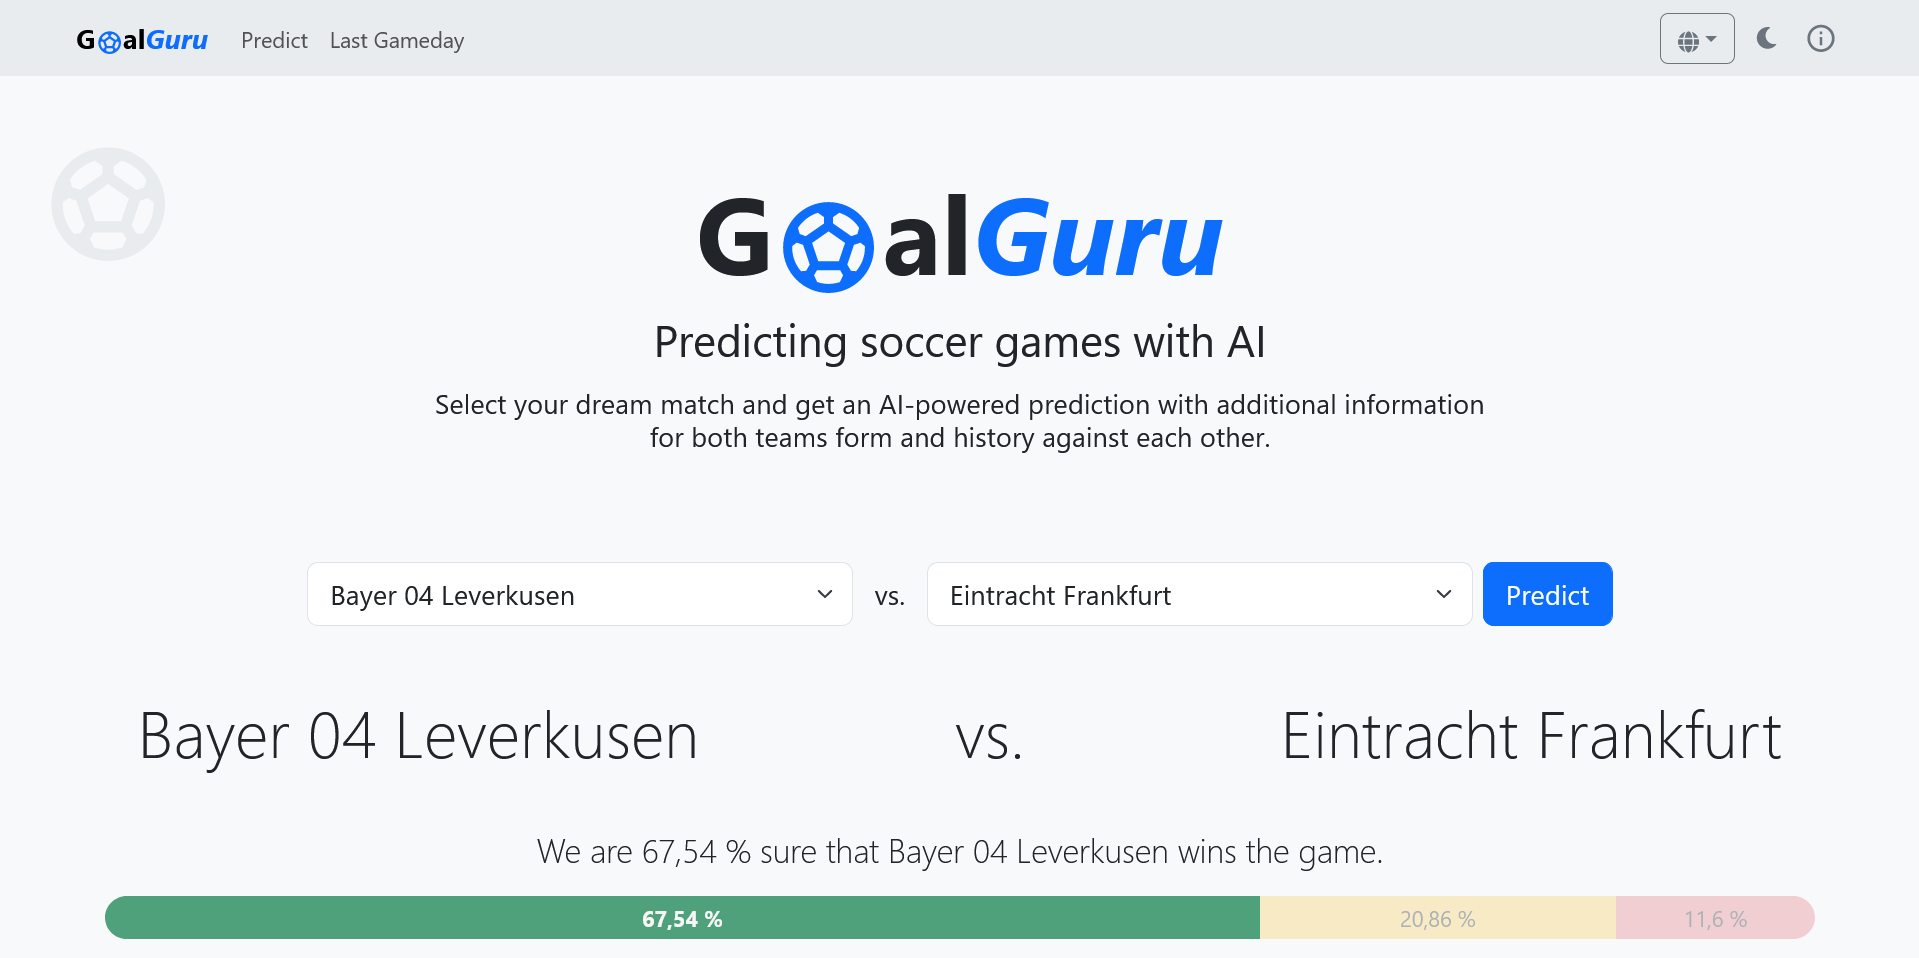
\includegraphics[width=1\textheight]{Screenshot 2024-06-28 at 13-46-20 GoalGuru.png}
    \caption{The GoalGuru frontend main route with a prediction for a game between \textquote{Bayer 04 Leverkusen} vs. \textquote{Eintracht Frankfurt} (the additional team information is located below the shown area)}
    \label{fig:goalgurufrontend}
\end{sidewaysfigure*}


\end{document}
